% Drawing 154/06-29 -- folder 154, batch 06, archive page 113 (PDF page 114).
% Transcription: au-dessous, au crayon, un cercle traversé de courbes
% Kind: pencil circle crossed by curves. Method 2 (schematic redraw from the facsimile). Status: ok.
% Notes: Pencil circle; a thin spindle across it from the upper left to the lower right, both sides meeting at a point of the upper left rim and at a point just outside the lower right rim, one side starting a little before the rim and running a little beyond it; a second thin spindle from the top of the rim to the bottom (the transcription's « traversé de courbes »); a short hook inside the left rim and a short stroke inside the lower left rim. Overlaid on the 400 dpi colour crop on 2026-11-12 and redrawn: the earlier redraw had one curve from top to bottom where the page has a spindle, and the first spindle 3 to 5 mm off. Redrawn 2026-11-12 (issue 128): to check again. Overlay check 2026-11-13 (issue 128, Claude claude-opus-5-5): redraw compiled with tectonic and laid over the 402 ppi scan; every stroke was about 1 to 1.5 mm above the ink and the circle was a regular oval where the page's is flattened at the lower right. Retraced from a millimetre grid on the crop: the circle through 30 points of the page, the two thick strokes of the oblique spindle (from (25,-17.1) to (85.9,-57.5) and from (31.6,-13.5) to the lower right point (81.4,-54.1)), the vertical spindle from (54.3,-13.4) to (50.9,-78.5), the hook inside the left rim and the stroke inside the lower left rim. Now matches the facsimile.
% Coordinates: 1 unit = 1 mm = 1/100 of the crop width (bbox in page fractions: [0.7, 0.185, 0.84, 0.275]).
% Redrawn by Claude (claude-fable-5-2), issue #128, 2026-11-12; not checked by a human; not compiled (no TeX in the session).
% Corrected by Claude (claude-fable-5-2) 2026-11-12 (issue #128): overlaid on the 400 dpi colour facsimile and redrawn from it (the second spindle, the two short strokes; the first spindle and the circle placed on the pencil). Not compiled. Status: ok.
% Checked by Claude (claude-opus-5-5) 2026-11-13 (issue #128): overlay on the 402 ppi colour facsimile, corrected, compiled with tectonic. Not checked by a human. Status: ok.
% Rights: reproduces part of the work -- behind RENDER_TRANSCRIPTS, never published by itself.
\documentclass[tikz,border=3pt]{standalone}
\usepackage{amsmath,amssymb}
\usetikzlibrary{patterns,arrows.meta}
\tikzset{pencil/.style={black!45}, struck/.style={black!35}, mpt/.style={circle,draw,inner sep=1.3pt}, pt/.style={circle,fill,inner sep=0.9pt}, opt/.style={circle,draw,fill=white,inner sep=1.1pt}}
\begin{document}
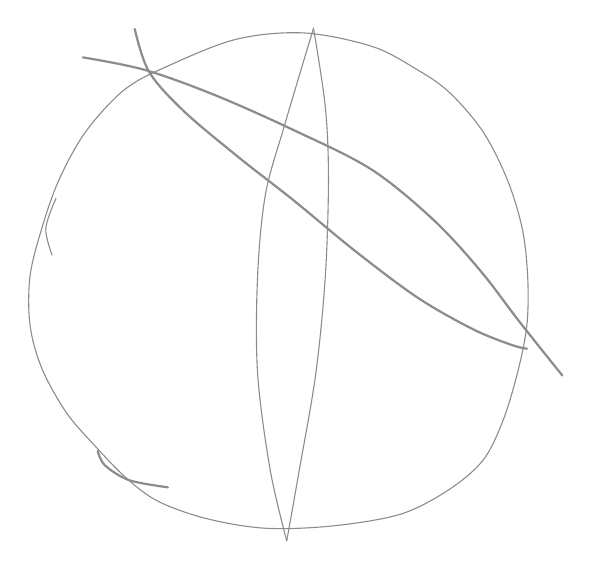
\begin{tikzpicture}[x=1mm,y=1mm,line cap=round,line join=round,font=\scriptsize]
\draw[pencil] plot[smooth cycle, tension=0.55] coordinates {(53.1,-14) (44.5,-14.8) (35.8,-18.2) (30.3,-21.2) (25.4,-26.5) (22,-32.6) (19.8,-38.8) (18.3,-44.9) (18.3,-51.1) (19.8,-56.6) (22.9,-62.2) (26.6,-66.5) (30.5,-70.5) (34.6,-73.5) (40.8,-75.7) (48.2,-76.9) (56.8,-76.6) (65.4,-75.1) (71.5,-72) (75.8,-68.3) (78.3,-63.4) (80.2,-57.2) (81.4,-51.1) (81.5,-44.9) (80.8,-38.8) (78.9,-32.6) (75.8,-26.5) (71.5,-21.5) (67.2,-18.5) (61.7,-15.7)};
\draw[pencil,thick] plot[smooth, tension=0.55] coordinates {(25,-17.1) (32.9,-18.7) (41.8,-21.9) (51.7,-26.3) (61.6,-31.3) (69.5,-37.7) (75.5,-44.2) (80.4,-50.6) (85.9,-57.5)};
\draw[pencil,thick] plot[smooth, tension=0.55] coordinates {(31.6,-13.5) (33.4,-18.9) (37.8,-23.9) (44.8,-29.8) (51.7,-35.2) (59.6,-41.7) (67.5,-47.6) (74.5,-51.6) (79.4,-53.6) (81.4,-54.1)};
\draw[pencil] plot[smooth, tension=0.55] coordinates {(54.3,-13.4) (50.6,-25.8) (48.2,-34.5) (47.2,-44.9) (47.2,-57.2) (48.8,-69.5) (50.9,-78.5)};
\draw[pencil] plot[smooth, tension=0.55] coordinates {(54.3,-13.4) (55.8,-23.4) (56.2,-32.6) (55.8,-44.9) (54.6,-57.2) (52.5,-69.5) (50.9,-78.5)};
\draw[pencil] plot[smooth, tension=0.55] coordinates {(21.6,-35) (20.3,-38.8) (21.1,-42.2)};
\draw[pencil,thick] plot[smooth, tension=0.55] coordinates {(26.9,-67.1) (27.8,-68.9) (30.9,-70.8) (35.8,-71.7)};
\end{tikzpicture}
\end{document}
